\section{Funding model and sustainability}

The \pmu will benefit from a diverse funding model that includes institutional support, competitive research grants, and strategic partnerships with industry leaders. This multifaceted approach provides a robust financial foundation that helps ongoing research and development in paediatric precision medicine. Institutional support from Kispi and its affiliated academic entities should furnish a stable base of funding that sustains core facilities and staffing requirements.

Beyond traditional funding avenues, we may proactively establishes collaborations with pharmaceutical companies and biotechnology firms. These partnerships frequently catalyse joint research projects and grant access to avant-garde technologies and additional streams of funding. By harmonising our research objectives with the needs of our industry partners, we not only secure essential resources but also ensure that our research outputs are pragmatically applicable and rapidly translatable into clinical settings.

Furthermore, we are dedicated to integrating sustainable practices to sustain all facets of our research activities, from data management and analysis to  resource utilisation. Our goal is to build a system that is redundant to decay. To do so, we must produce tools that are sensible for newcomers to learn, provide a consistent method of production and usage so that they can be updated and maintained without dependency on single members. 

The most common research funding pathways for academic members of the \pmu are shown in 
\textbf{figure
\ref{fig:Research_Funding_Pathways}} 
and links to funding opportunities that are also supported by UZH assistance are provided in 
\textbf{table
\ref{tab:funding_opportunities}}.

\begin{figure}[h] \hspace*{0cm} 
\begin{center}
	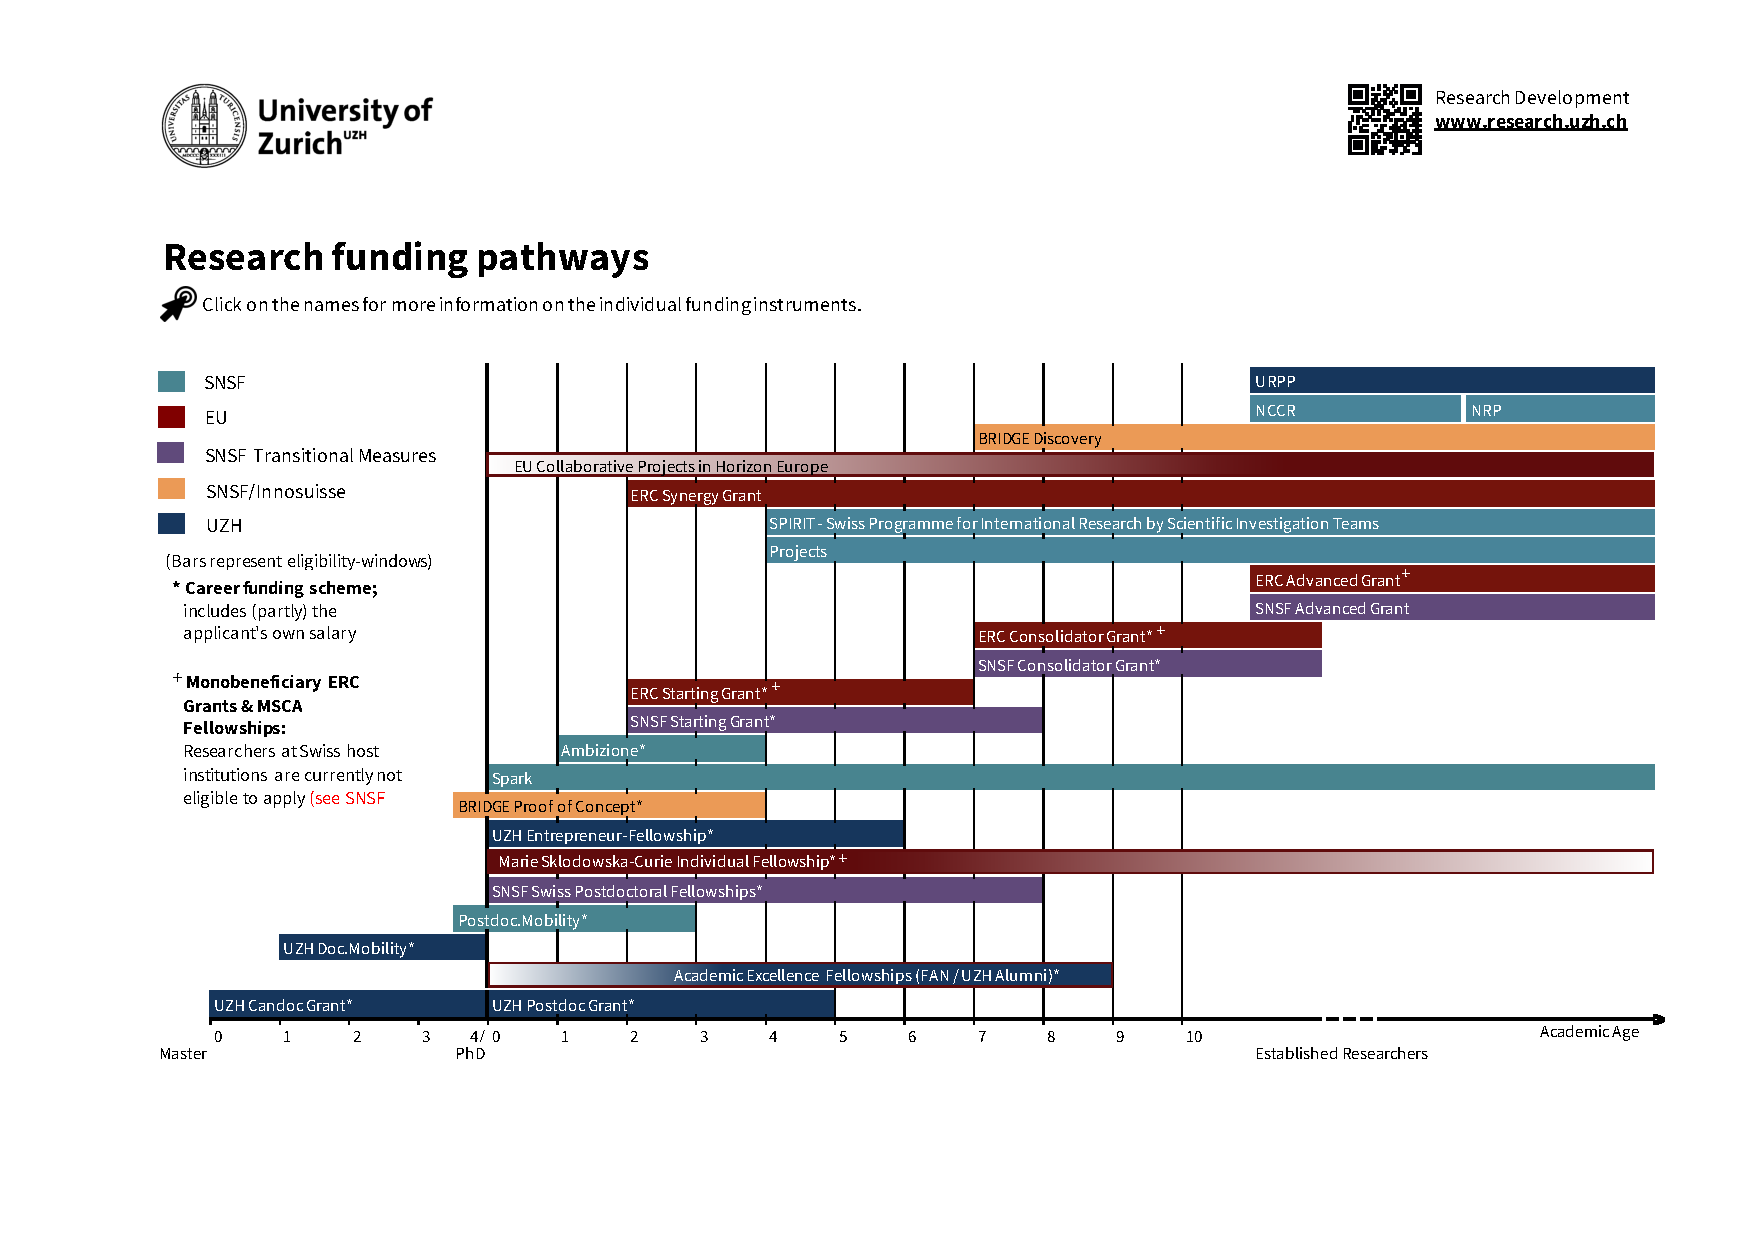
\includegraphics[width=0.98\textwidth]{Research_Funding_Pathways}
	\caption{Most common research funding pathways for academic members.}
	\label{fig:Research_Funding_Pathways}
\end{center}
\end{figure}

\begin{table}[ht] \hspace*{-5em} 
\centering
\begin{tabular}{ll}
\hline
\multicolumn{2}{c}{Program} \\
\hline
\href{https://uzhalumni.ch/page/alumnifonds?lang=en}{Alumni-Fonds, UZH} & \href{https://www.research.uzh.ch/en/funding/postdoc/prima.html}{PRIMA (Promoting Women in Academia, SNSF)} \\
\href{https://www.research.uzh.ch/en/funding/postdoc/ambizione.html}{Ambizione (SNSF)} & \href{https://www.research.uzh.ch/en/funding/researchers/pd-stiftung.html}{Privatdozenten-Stiftung, UZH} \\
\href{https://www.research.uzh.ch/en/funding/postdoc/axa.html}{AXA Research Fund} & \href{http://www.snf.ch/en/funding/infrastructures/requip/Pages/default.aspx}{Research Equipment (R’Equip, SNSF)} \\
\href{https://www.innovation.uzh.ch/en/entrepreneur-guide/funding/bridge-snf-innosuisse.html}{Bridge: Discovery} & \href{http://www.snf.ch/en/funding/science-communication/scientific-exchanges/Pages/default.aspx}{Scientific Exchanges (SNSF)} \\
\href{https://www.innovation.uzh.ch/en/entrepreneur-guide/funding/bridge-snf-innosuisse.html}{Bridge: Proof of Concept} & \href{https://snis.ch/funding/}{SNIS Project Funding} \\
\href{https://www.research.uzh.ch/en/funding/researchers/competence.html}{Centers of Competence} & \href{https://www.research.uzh.ch/en/funding/researchers/SNSF-Advanced-Grant.html}{SNSF Advanced Grant} \\
\href{https://www.citizenscience.uzh.ch/en/services/seedgrants.html}{Citizen Science Seed Grants (UZH)} & \href{https://www.research.uzh.ch/en/funding/postdoc/SNSF-Consolidator-Grant.html}{SNSF Consolidator Grant} \\
\href{https://collegium.ethz.ch/fellowships/early-career-fellowship}{Collegium Helveticum Early-Career Fellowships} & \href{https://www.research.uzh.ch/en/funding/postdoc/eccellenza-fellowships.html}{SNSF Eccellenaz Professorial Fellowship} \\
\href{https://collegium.ethz.ch/fellowships/senior-fellowship}{Collegium Helveticum Senior Fellowships} & \href{https://www.research.uzh.ch/en/funding/researchers/snf-projekte.html}{SNSF Project Funding} \\
\href{https://www.research.uzh.ch/en/funding/researchers/forschungssemester.html}{Competitive Sabbaticals, UZH} & \href{https://www.research.uzh.ch/en/funding/postdoc/SNSF-Starting-Grant.html}{SNSF Starting Grant} \\
\href{https://www.swissuniversities.ch/en/topics/promotion-of-young-talent/cotutelles-de-these}{Cotutelle de Thèse} & \href{https://www.research.uzh.ch/en/funding/postdoc/SNSF-Swiss-Postdoctoral-Fellowship.html}{SNSF Swiss Postdoctoral Fellowship} \\
\href{https://dizh.ch/en/activities/innovationprogram/}{DIZH Innovation Program} & \href{https://www.research.uzh.ch/en/funding/postdoc/spark.html}{Spark (SNSF)} \\
\href{https://www.dsi.uzh.ch/de/research/funding/infrastructure-lab.html}{DSI Infrastructure \& Lab Call} & \href{https://sphn.ch/}{SPHN (Swiss Personalized Health Network)} \\
\href{https://www.research.uzh.ch/en/funding/researchers/ERC-Advanced-Grant.html}{ERC Advanced Grant} & \href{https://www.research.uzh.ch/en/funding/researchers/spirit.html}{SPIRIT (SNSF)} \\
\href{https://www.research.uzh.ch/en/funding/postdoc/erc.html}{ERC Grants} & \href{https://www.research.uzh.ch/en/funding/researchers/3rcc.html}{Swiss 3R Competence Centre (3RCC) } \\
\href{https://www.fan4talents.uzh.ch/de.html}{FAN Academic Excellence Fellowships, UZH} & \href{https://www.sbfi.admin.ch/sbfi/en/home/education/scholarships-and-grants/swiss-government-excellence-scholarships.html}{ Excellence Scholarships for Foreign Scholars} \\
\href{https://www.swissuniversities.ch/en/service/scholarships-for-study-abroad/government-scholarships}{Foreign Government Scholarships} & \href{https://research.swiss/}{ Research and Innovation Cooperation Programs} \\
\href{https://www.research.uzh.ch/en/funding/researchers/stwf.html}{Foundation for Research in Science and the Humanities at UZH} & \href{https://sphn.ch/}{Swiss Personalized Health Network (SPHN)} \\
\href{https://www.grc.uzh.ch/en/funding/grc-new-grants.html}{GRC Grants (UZH)} & \href{https://www.int.uzh.ch/en/out/program/erasmus.html}{Swiss-European Mobility Programme} \\
\href{https://www.grc.uzh.ch/de/funding/grc-new-grants.html}{GRC Travel Grant (UZH)} & \href{https://www.swissuniversities.ch/en/organisation/projects-and-programmes/}{swissuniversities: Project Contributions} \\
\href{https://gspi.ch/icp/}{GSPI Impact Collaboration Programme} & \href{https://www.research.uzh.ch/en/funding/researchers/transform.html}{TRANSFORM (UZH)} \\
\href{https://www.kispi.uzh.ch/forschungszentrum/nachwuchsfoerderung}{Heidi Ras} & \href{https://www.research.uzh.ch/en/funding/researchers/UFSP.html}{University Research Priority Programs (URPP)} \\
\href{https://grantsaccess.ethz.ch/de/horizon-europe.html}{Horizon Europe} & \href{https://www.research.uzh.ch/en/funding/phd/uzhcandoc.html}{UZH Candoc Grant} \\
\href{https://www.research.uzh.ch/en/funding/researchers/innosuisse.html}{Innosuisse Projects} & \href{https://www.research.uzh.ch/en/funding/phd/uzh-doc-mobility.html}{UZH Doc.Mobility} \\
\href{https://grantsaccess.ethz.ch/find/most-common-eu-programs/msca-pf.html}{Marie Skłodowska-Curie Postdoctoral Fellowships} & \href{https://www.research.uzh.ch/en/funding/postdoc/entrepreneur-fellowships.html}{UZH Entrepreneur Fellowships} \\
\href{https://www.research.uzh.ch/en/funding/researchers/NCCR.html}{National Centers of Competence in Research (NCCR)} & \href{https://www.global.uzh.ch/en/networks/funding-instruments/partnerships-fund.html}{UZH Global Strategy and Partnerships Funding Scheme} \\
\href{http://www.snf.ch/en/funding/programmes/national-research-programmes-nrp/Pages/default.aspx}{National Research Programmes (NRP)} & \href{https://www.research.uzh.ch/static/fnf/stiftungen/}{UZH Index of Foundations (German only)} \\
\href{https://grantsaccess.ethz.ch/submit/us-funding.html}{NIH and other US Grants} & \href{https://www.research.uzh.ch/en/funding/postdoc/uzhpostdoc.html}{UZH Postdoc Grant} \\
\href{https://www.research.uzh.ch/en/funding/postdoc/postdoc-mobility.html}{Postdoc.Mobility (SNSF)} & \href{ }{ }\\
\hline
\end{tabular}
\caption{List of funding opportunities which include organisational support by UZH. (Note hyper-links in electronic PDF version.)}
\label{tab:funding_opportunities}
\end{table}

\clearpage


